% !TEX encoding = UTF-8
% !TEX TS-program = pdflatex
% !TEX root = ../tesi.tex

%**************************************************************
\chapter{Descrizione dello Stage}
\label{cap:descrizione-stage}
%**************************************************************

% \intro{Brevissima introduzione al capitolo}

%**************************************************************
\section{Scelta dello Stage}

La scelta dello stage è stata molto difficile. Ero alla ricerca, infatti, di un contesto specifico per la mia prima esperienza lavorativa
nel settore informatico. Consultando tutte le varie proposte, durante l'evento Stage-IT, ho fatto fatica a trovare una proposta che mi
convincesse a fondo. Alcune delle aziende che ho contattato si sono dimostrate disponibili nei miei confronti, ma per le
tempistiche legate alla laura ho dovuto rinunciare alle loro proposte.
%  Tra le motivazioni per le quali ho scelto \gls{asd} c'è senz'altro un progetto chiaro e
% stimolante, ma anche la disponibilità immediata allo stage.

\subsection{Motivazioni della scelta}

Quello di cui ero alla ricerca era un contesto piccolo con ampi margini di crescita e di formazione personale sulle tecnologie moderne, più
che sul metodo di lavoro, che invece tende a essere molto più definito in aziende grandi, con un modello affermato e utilizzato da tempo.
Quello che mi interessava era sperimentare vari ruoli, comprendere le varie responsabilità che questi comportano e come interfacciarsi con
altri dipendenti. \\
Oltre al contesto aziendale ero attratto anche dall'argomento del progetto. Volevo sperimentare nuove tecnologie e nuovi linguaggi,
disegnare e creare del software, piuttosto che mantenerlo o estenderlo. Da questo punto di vista l'Università di Padova,
attraverso Stage-IT mi ha messo in contatto con molte aziende interessanti. Inoltre la mia ricerca del progetto di stage si è basata sul desiderio
di lavorare in ambito frontend e questo ha ristretto di molto le varie opportunità. \\
Il fattore decisivo sulla scelta dello stage è stato il fatto che da tempo volevo sperimentare le tecnologie per lo sviluppo di applicazioni
mobile. Io stesso, precedentemente, avevo provato ad avviare qualche piccolo progetto in questo campo e per questo ho voluto
scegliere una proposta che avesse questo come tema principale. \\
In questo senso l'offerta di \acrlong{asd} ha subito catturato la mia attenzione e nonostante fosse la loro prima esperienza con uno
studente laureando, ho preso contatti per avviare con loro il mio stage.

\subsection{Obiettivi personali}
\label{sec:obiettivi-pers}
Le esperienze lavorative precedenti a questa mi avevano insegnato cosa vuol dire lavorare in una squadra e cos'è prendersi carico
di responsabilità, ma con nessuna di queste avevo messo in pratica ciò che avevo studiato finora. Sentivo quindi il bisogno di consolidare
il bagaglio di nozioni acquisite durante gli anni del corso e lo stage ne è stata l'occasione perfetta. Certo, ci sono stati i molteplici
progetti didattici, ma nulla è come entrare nel contesto lavorativo e avere contatto diretto con questa realtà. \\
Principalmente le mie aspirazioni si possono riassumere in:
\begin{itemize}
	\item collaborare con colleghi con molta più esperienza e conoscenza di me;
	\item imparare nuove tecnologie e distinguere quelle buone da quelle cattive;
	\item migliorare la mia gestione del tempo e organizzarmi con le scadenze dei vari compiti;
	\item trovare proposte e contatti per progetti futuri.
\end{itemize}

%**************************************************************

\section{La proposta di stage}

\acrlong{asd} ha aperto una posizione per uno stage a una persona interessata al mobile development, che potesse collaborare sia nella parte di analisi, che nella parte di codifica. Il progetto era incentrato sulla formazione sulle tecnologie mobile, per fare evolvere l'azienda anche su questo ramo cercando nuove opportunità.

\subsection{Il contesto}

Come già accennato {\hyperref[cap:introduzione]{nel primo capitolo}} Alternative Studio è un'azienda giovane che da 5 anni collabora con
\gls{ucis}. Durante questi anni è stato sviluppato un gestionale e un sito per la loro organizzazione.

% chiedere info sul gestionale

All'interno di questo gestionale è stata sviluppata un'\acrshort{api}, volta alla registrazione di log contenenti la posizione tramite
coordinate e alla creazione di una relativa traccia. A questo software attualmente si interfaccia un'applicazione sviluppata 5 anni fa, non
da \acrlong{asd}, e pubblicata nel 2018 con il nome di UCIS Report Tool. L'applicazione ha come funzionalità principale la creazione e la
gestione di attività, con la registrazione e l'invio di log contenenti la posizione del dispositivo sul quale esegue. Questa, però, non
risulta essere un prodotto professionale e utilizza tecnologie già vecchie e difficilmente manutenibili o aggiornabili. Inoltre sono stati
lamentati da \gls{ucis} alcuni bug e pochissima precisione nella registrazione della posizione. Dall'associazione nasce così l'esigenza di aggiornare
o riscrivere completamente l'applicazione. \\
\noindent Alternative Studio ha colto, quindi, l'opportunità di sviluppare una sua versione dell'applicativo e di proporlo poi all'organizzazione con la quale già collabora.

\subsubsection{Problematiche dell'applicazione UCIS Report Tool}
L'applicazione attualmente utilizzata da UCIS è stata sviluppata interamente in linguaggio nativo, esclusivamente per il
sistema operativo \gls{Android}. Il principale problema rimane in ogni caso la scarsa precisione nella lettura delle
tracce GPS. L'invio dei log e troppo dilazionato nel tempo rendendo la traccia risultante frastagliata e alle volte
incomprensibile. Essendo la funzione primaria questo risulta essere un grosso problema, ma non è certamente l'unico. La
disposizione delle viste non è logica e lascia l'utente disorientato. Inoltre i form risultano essere errati: alcune
delle opzioni non devono essere presenti e la selezione di una non provoca effetti su un'altra. Ad esempio se volessi
creare una nuova attività dovrei selezionare la macrocategoria e di conseguenza filtrare la selezione della categoria
successiva. Ciò non avviene e provoca un'errore nell'invio del form. \\
\noindent Forse il problema più grande è la non manutenibilità di questo software. Il codice risulta poco modulare e la
lettura delle classi ostica. È privo di documentazione formale e di una progettazione sensata. Risulta essere un
prodotto morto e non professionale. \\
\noindent Un altro punto negativo dell'applicazione è il kit grafico utilizzato, risulta essere vecchio e di sicuro non
accattivante per l'utente e meno ancora per il cliente.

\subsection{Obiettivi dello stage}
\label{sec:obiettivi}

Durante la compilazione del Piano di Lavoro, documento che mette in chiaro ciò che andrà fatto durante lo stage, con il tutor sono stati fissati gli obiettivi principali dello stage, che qui sono elencati e raggruppati come obbligatori, desiderabili e facoltativi.

\begin{itemize}
	\item Obbligatori
	\begin{itemize}
		\item progettazione e realizzazione di applicazione mobile;
    \item implementare servizio di geolocalizzazione preciso nell’applicazione;
    \item versione beta da pubblicare sullo store.
	\end{itemize}

	\item Desiderabili
	\begin{itemize}
		\item applicazione cross-platform, combatibile anche su dispositivi datati;
    \item messa in produzione dell’applicazione.
	\end{itemize}

	\item Facoltativi
	\begin{itemize}
		\item implementazione delle notifiche push;
    \item integrazione di una chat;
    \item applicazione funzionante anche su dispositivi senza servizi Google.
	\end{itemize}
\end{itemize}

\subsection{Pianificazione}

In seguito si è discusso su come ripartire le ore e decidere quali processi mi avrebbero portato a soddisfare gli obiettivi sopra scritti.
Si è prodotta una pianificazione oraria che prevedeva gran parte della prima parte dello stage in formazione e creazione di una \gls{product
baseline} e una seconda parte di codifica e testing dell'applicazione, per chiudere con il collaudo e la pubblicazione sullo store Android.
\\
Il progetto di stage prevedeva circa 320 ore e in particolare si era stimata la durata delle varie attività:
\begin{itemize}
		\item \textbf{Prima Settimana}
		\begin{itemize}
				\item Analisi e formazione delle tecnologie da utilizzare nel progetto;
				\item studio del framework ionic;
				\item studio di geolocalizzazione;
				\item studio per notifiche push.
		\end{itemize}
		\item \textbf{Seconda Settimana}
		\begin{itemize}
			\item Prototipo applicazione funzionante;
			\item implementazione funzionalità di gestione delle utenze;
			\item navigazione tra schermate dell’app.
		\end{itemize}
		\item \textbf{Terza Settimana}
		\begin{itemize}
				\item implementazione registrazione delle attività.
		\end{itemize}
		\item \textbf{Quarta Settimana}
		\begin{itemize}
				\item implementazione del salvataggio offline dei dati.
		\end{itemize}
		\item \textbf{Quinta Settimana}
		\begin{itemize}
				\item aggiunta chiamante API al gestionale.
		\end{itemize}
		\item \textbf{Sesta Settimana}
		\begin{itemize}
				\item implentazione gestione emergenze.
				\item test.
		\end{itemize}
		\item \textbf{Settima Settimana}
		\begin{itemize}
				\item collaudo;
				\item messa in produzione.
		\end{itemize}
		\item \textbf{Ottava Settimana}
		\begin{itemize}
				\item aggiunta requisiti facoltativi.
		\end{itemize}
\end{itemize}

I dettagli sono riportati sul seguente \gls{diagramma di Gantt}.

\begin{figure}[h]
	\begin{center}
		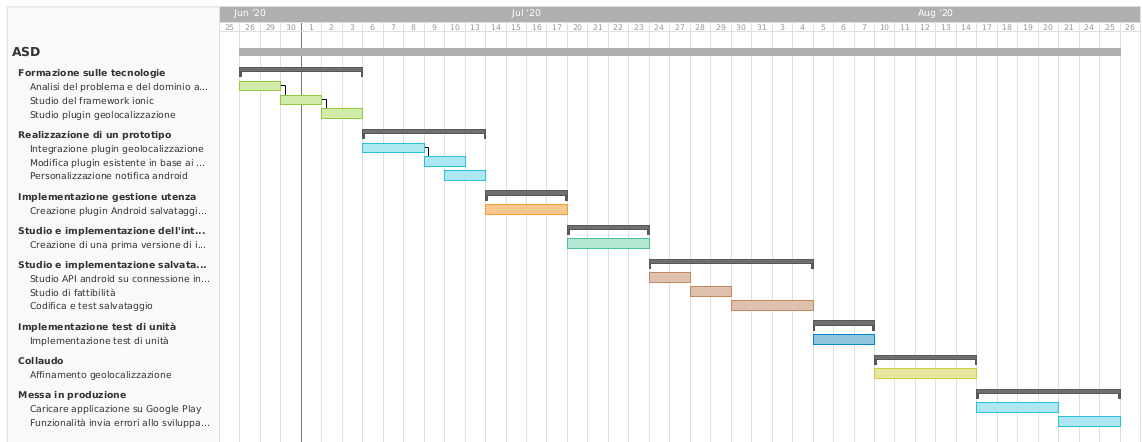
\includegraphics[height=6cm]{gantt}
		\caption{\Gls{diagramma di Gantt} della ripartizione giornaliera.}
	\end{center}
\end{figure}

\subsection{Vincoli}

Questo capitolo si occupa di descrivere i vincoli ai quali sono stato sottoposto durante lo stage. Tengo a precisare che quelli imposti dall'azienda non sono mai stati un ostacolo, bensì delle guide precise per raggiungere al meglio gli obiettivi. I vincoli sono stati raggruppati nelle sezioni successive.

\subsubsection{Vincoli tecnologici}
Il vincolo più importante imposto è stato quello di non scrivere l'applicazione in linguaggio nativo per ogni sistema operativo. Nonostante
sia stata sviluppata solamente per il sistema operativo Android, l'idea iniziale era quella di produrla \gls{crossplatform} e di portarla con
poche modiche su qualunque sistema operativo mobile e non. È per questo che il tutor mi ha imposto la ricerca di un framework ibrido.

\subsubsection{Vincoli metodologici}
Il mio stage si è svolto, purtropp o, durante un periodo soggetto a restrizioni negli spostamenti dovuti all'epidemia di SARS-CoV-2. Dopo un
periodo iniziale, però, sono riuscito a svolgere lo stage in parte in presenza. Quinid ho concordato con il tutor di poter accedere ai locali di
Alternative Studio almeno due giorni a settimana, solitamente il lunedì e il venerdì. \\
Per quanto riguarda il metodo di lavoro ho cercato diverse volte consiglio presso il tutor. Riuscire a svolgere lo stage in presenza, anche
se in parte, è stato molto importante in questo senso. Infine per aderire in parte al metodo \gls{Agile} abbiamo organizzato una breve riunione
giornaliera, che aveva come scopo quello di allineare il lavoro e programmare le tasks successive.

\subsubsection{Vincoli temporali}
Oltre al vincolo di 320 ore, imposto dalla natura dello stage e dall'azienda stessa, sono dovuto sottostare alle scadenze delle varie tasks
impostate su Gitlab. In particolare si è scelto di lavorare 40 ore alla settimana. \\
Non essendo stato  uno stage completamente in presenza, non si è dato nessun vincolo sulla singola giornata lavorativa. Solitamente l'orario
lavorativo iniziava alle 9:00 e si concludeva alle 18, con un'ora di pausa pranzo. Questo per me è stato un problema da affrontare, perché
ho notato che sono molto più produttivo quando ho delle restrizioni sugli orari. Il problema è stato fatto presente al tutor che ha
collaborato nel controllo e nel conteggio delle ore effettiva di lavoro.
